% =====================================================================
%  Figure 1 -- Example for the 3DP-CPTP
%  Left  : routing plan of the two vehicles over the customer graph
%  Right : three-dimensional packing inside the first vehicle
%
%  Compile with pdflatex / lualatex (needs pgfplots >= 1.16)
% =====================================================================
\documentclass[tikz,border=5pt]{standalone}

\usepackage{tikz}
\usepackage{pgfplots}
\pgfplotsset{compat=1.18}
\usetikzlibrary{calc,positioning,3d}

% --- matplotlib default colour cycle -------------------------------
\definecolor{mplblue}  {HTML}{1F77B4}   % vehicle 1
\definecolor{mplorange}{HTML}{FF7F0E}   % vehicle 2

% --- colours of the packed items -----------------------------------
\definecolor{itemA}{HTML}{4C72B0}
\definecolor{itemB}{HTML}{DD8452}
\definecolor{itemC}{HTML}{C44E52}
\definecolor{itemD}{HTML}{8172B3}
\definecolor{itemI}{HTML}{64B5CD}

% =====================================================================
%  Isometric projection macro for the packing drawing
%    \bx{x}{y}{z}{dx}{dy}{dz}{colour}{label}
%  Axes:  x to the upper left, y to the upper right, z upwards.
%  The origin (0,0,0) is the near bottom corner of the container.
% =====================================================================
\newcommand{\isox}{-0.62}   % screen x per unit of model x
\newcommand{\isoy}{ 0.32}   % screen y per unit of model x
\newcommand{\jsox}{ 0.62}   % screen x per unit of model y
\newcommand{\jsoy}{ 0.32}   % screen y per unit of model y
\newcommand{\ksoy}{ 1.00}   % screen y per unit of model z

% project a model point (#1,#2,#3) to screen coordinates
\newcommand{\pt}[3]{%
  ({\isox*(#1)+\jsox*(#2)},{\isoy*(#1)+\jsoy*(#2)+\ksoy*(#3)})}

% label offset applied to the next \bx (reset automatically afterwards)
\def\bxlx{0pt}\def\bxly{0pt}
\newcommand{\nudge}[2]{\global\def\bxlx{#1}\global\def\bxly{#2}}

% one axis-aligned box: origin (#1,#2,#3), size (#4,#5,#6), colour #7, label #8
\newcommand{\bx}[8]{%
  \begin{scope}[every path/.style={draw=#7!65!black,line join=round}]
    % --- right-hand face  (y = #2, points towards the viewer) ------
    \fill[#7,fill opacity=.55]
      \pt{#1}{#2}{#3} -- \pt{#1}{#2+#5}{#3}
      -- \pt{#1}{#2+#5}{#3+#6} -- \pt{#1}{#2}{#3+#6} -- cycle;
    \draw
      \pt{#1}{#2}{#3} -- \pt{#1}{#2+#5}{#3}
      -- \pt{#1}{#2+#5}{#3+#6} -- \pt{#1}{#2}{#3+#6} -- cycle;
    % --- left-hand face   (x = #1, points towards the viewer) ------
    \fill[#7,fill opacity=.45]
      \pt{#1}{#2}{#3} -- \pt{#1+#4}{#2}{#3}
      -- \pt{#1+#4}{#2}{#3+#6} -- \pt{#1}{#2}{#3+#6} -- cycle;
    \draw
      \pt{#1}{#2}{#3} -- \pt{#1+#4}{#2}{#3}
      -- \pt{#1+#4}{#2}{#3+#6} -- \pt{#1}{#2}{#3+#6} -- cycle;
    % --- top face (z = const) --------------------------------------
    \fill[#7,fill opacity=.65]
      \pt{#1}{#2}{#3+#6} -- \pt{#1+#4}{#2}{#3+#6}
      -- \pt{#1+#4}{#2+#5}{#3+#6} -- \pt{#1}{#2+#5}{#3+#6} -- cycle;
    \draw
      \pt{#1}{#2}{#3+#6} -- \pt{#1+#4}{#2}{#3+#6}
      -- \pt{#1+#4}{#2+#5}{#3+#6} -- \pt{#1}{#2+#5}{#3+#6} -- cycle;
  \end{scope}
  % --- item number, centred on the top face ------------------------
  %     a white halo keeps it readable where boxes overlap
  \node[font=\scriptsize,text=black,inner sep=1pt,
        fill=white,fill opacity=.72,text opacity=1,rounded corners=1pt,
        xshift=\bxlx,yshift=\bxly]
    at \pt{#1+0.5*#4}{#2+0.5*#5}{#3+#6} {#8};
  \global\def\bxlx{0pt}\global\def\bxly{0pt}%
}

\begin{document}
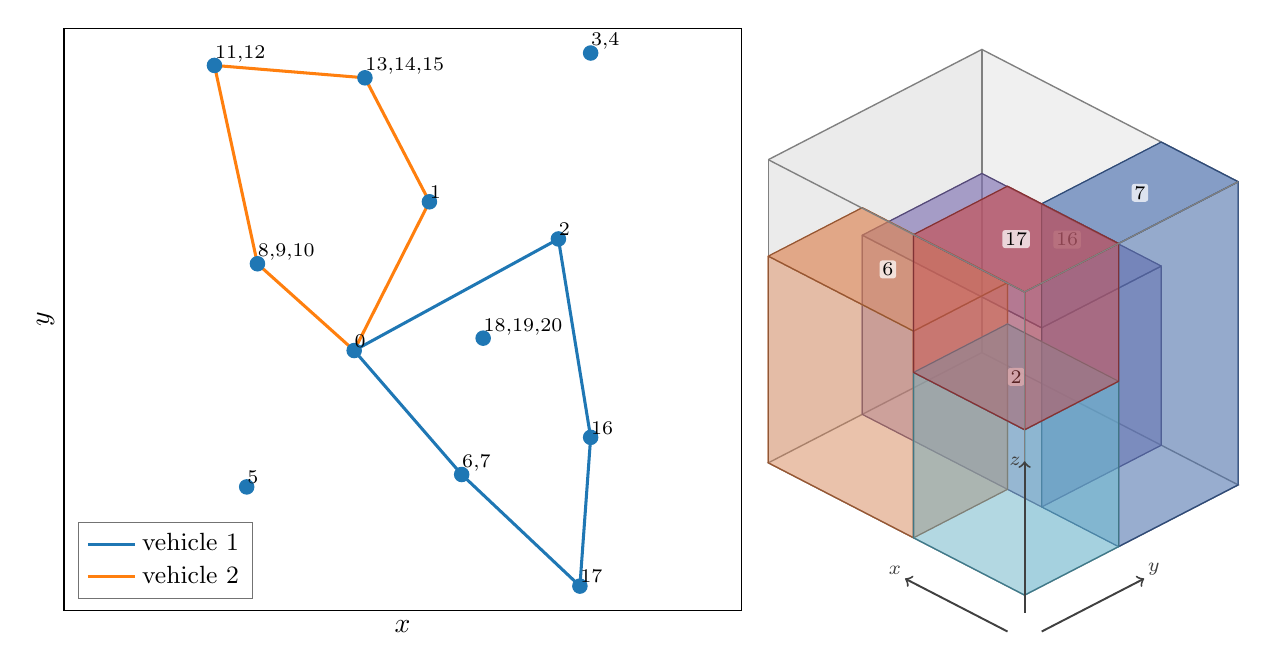
\begin{tikzpicture}

% =====================================================================
%  (a)  Routing part
% =====================================================================
\begin{scope}
\begin{axis}[
    name=routes,
    width=8.6cm, height=7.4cm,
    scale only axis,
    xlabel={$x$}, ylabel={$y$},
    xmin=3, xmax=66, ymin=19, ymax=66,
    xtick=\empty, ytick=\empty,
    axis line style={black},
    legend style={
        at={(0.02,0.02)}, anchor=south west,
        draw=black!55, fill=white, font=\small,
        cells={anchor=west},
    },
    legend cell align=left,
]

% ---- tour of vehicle 1 : 0 - 2 - 16 - 17 - 6,7 - 0 ----------------
\addplot[mplblue,line width=1.1pt,mark=none] coordinates {
    (30,40) (49,49) (52,33) (51,21) (40,30) (30,40)
};
\addlegendentry{vehicle 1}

% ---- tour of vehicle 2 : 0 - 1 - 13,14,15 - 11,12 - 8,9,10 - 0 ----
\addplot[mplorange,line width=1.1pt,mark=none] coordinates {
    (30,40) (37,52) (31,62) (17,63) (21,47) (30,40)
};
\addlegendentry{vehicle 2}

% ---- customers / depot -------------------------------------------
\addplot[
    only marks, mark=*, mark size=2.6pt,
    draw=mplblue, fill=mplblue,
    nodes near coords, point meta=explicit symbolic,
    every node near coord/.append style={
        anchor=south west, font=\scriptsize, text=black,
        inner sep=1pt, xshift=-1pt,
    },
] coordinates {
    (30,40) [0]
    (37,52) [1]
    (49,49) [2]
    (52,64) [3,4]
    (20,29) [5]
    (40,30) [6,7]
    (21,47) [8,9,10]
    (17,63) [11,12]
    (31,62) [13,14,15]
    (52,33) [16]
    (51,21) [17]
    (42,41) [18,19,20]
};

\end{axis}
\end{scope}

% =====================================================================
%  (b)  Three-dimensional packing inside vehicle 1
% =====================================================================
\begin{scope}[shift={($(routes.south east)+(3.6cm,0.2cm)$)},scale=0.175]

  % --- container D^x = 30, D^y = 25, D^z = 22 ----------------------
  \def\Dx{30}\def\Dy{25}\def\Dz{22}

  % ---- floor and the two far walls of the loading space -----------
  \fill[black!4]                                   % floor  (z = 0)
    \pt{0}{0}{0} -- \pt{\Dx}{0}{0} -- \pt{\Dx}{\Dy}{0} -- \pt{0}{\Dy}{0} -- cycle;
  \fill[black!8]                                   % far wall (x = Dx)
    \pt{\Dx}{0}{0} -- \pt{\Dx}{\Dy}{0} -- \pt{\Dx}{\Dy}{\Dz} -- \pt{\Dx}{0}{\Dz} -- cycle;
  \fill[black!6]                                   % far wall (y = Dy)
    \pt{0}{\Dy}{0} -- \pt{\Dx}{\Dy}{0} -- \pt{\Dx}{\Dy}{\Dz} -- \pt{0}{\Dy}{\Dz} -- cycle;

  \begin{scope}[draw=black!50,line width=.5pt]
    \draw \pt{0}{0}{0} -- \pt{\Dx}{0}{0} -- \pt{\Dx}{\Dy}{0} -- \pt{0}{\Dy}{0} -- cycle;
    \draw \pt{\Dx}{0}{0} -- \pt{\Dx}{0}{\Dz};
    \draw \pt{\Dx}{\Dy}{0} -- \pt{\Dx}{\Dy}{\Dz};
    \draw \pt{0}{\Dy}{0} -- \pt{0}{\Dy}{\Dz};
    \draw \pt{\Dx}{0}{\Dz} -- \pt{\Dx}{\Dy}{\Dz} -- \pt{0}{\Dy}{\Dz};
  \end{scope}

  % The five items carried by the FIRST vehicle: 2, 6, 7, 16, 17.
  % (Items 1, 8, 9, 10, 11, 12, 13, 14 and 15 travel in the second
  % vehicle; items 3, 4, 5, 18, 19 and 20 are rejected.)
  % Heterogeneous sizes, volume utilisation approx. 76%; no two items
  % overlap and every item lies completely inside the container.
  % Drawn far-to-near: descending (x+dx)+(y+dy), then ascending z, so
  % the painter's algorithm produces the correct occlusion.
  %
  %    \bx{x}{y}{z}{dx}{dy}{dz}{colour}{label}

  \nudge{20pt}{4pt}
  \bx{ 9}{11}{ 0}{21}{14}{13}{itemD}{16}
  \bx{13}{ 0}{ 0}{17}{11}{15}{itemB}{6}
  \bx{ 0}{11}{ 0}{ 9}{14}{22}{itemA}{7}
  \bx{ 0}{ 0}{ 0}{13}{11}{12}{itemI}{2}
  \bx{ 0}{ 0}{12}{13}{11}{10}{itemC}{17}

  % ---- near edges of the loading space (drawn last, on top) -------
  \begin{scope}[draw=black!50,line width=.5pt]
    \draw \pt{0}{0}{0} -- \pt{0}{0}{\Dz};
    \draw \pt{0}{0}{\Dz} -- \pt{\Dx}{0}{\Dz};
    \draw \pt{0}{0}{\Dz} -- \pt{0}{\Dy}{\Dz};
  \end{scope}

  % ---- axis indicators, drawn outside the container ---------------
  \begin{scope}[black!75,line width=.7pt,font=\scriptsize]
    \draw[->] \pt{0}{-2}{-2} -- \pt{12}{-2}{-2}
      node[pos=1,above left,inner sep=1pt]{$x$};
    \draw[->] \pt{-2}{0}{-2} -- \pt{-2}{12}{-2}
      node[pos=1,above right,inner sep=1pt]{$y$};
    \draw[->] \pt{-2}{-2}{0} -- \pt{-2}{-2}{11}
      node[pos=1,left,inner sep=1pt]{$z$};
  \end{scope}

\end{scope}

\end{tikzpicture}
\end{document}
